\section{Vision Transformer}

\begin{frame}[fragile]{Vision Transformer Architecture}
  \framesubtitle{Patch Embedding and Positional Econding}
  \textbf{Patch Embedding:}
  \begin{itemize}
    \item Converts images into \textbf{fixed size patches}.
    \item Each patch is flattened into a vector and projected into an \textbf{embedding space}.
      \begin{equation}
        X \in \mathbb{R}^{H \times W \times C} \quad \Rightarrow \quad N = \frac{H \times W}{P^2}
      \end{equation}
      \begin{equation}
        Z = [z_1, z_2, ..., z_N] \in \mathbb{R}^{N \times D}
      \end{equation}
  \end{itemize}

  \textbf{Positional Encoding:}
  \begin{itemize}
    \item Adds \textbf{spatial information} to the patches since transformers lack inherent \textbf{spatial bias}.
    \item Learnable positional embeddings:
      \begin{equation}
        Z_0 = Z + E_{pos}
      \end{equation}
  \end{itemize}
\end{frame}

\begin{frame}[fragile]{Vision Transformer Architecture}
  \framesubtitle{Transformer Encoder and Classification Head}
  \textbf{Transformer Encoder:}
  \begin{itemize}
    \item Processes the \textbf{sequence} of patch embeddings.
    \item Consists of multiple layers of \textbf{Multi Head Self Attention} (\textit{MHSA}) and \textbf{Feed Forward Networks} (\textit{FFN}).
      \begin{equation}
        FFN(z) = \text{GELU} (zW_1 + b_1) W_2 + b_2
      \end{equation}
      \begin{equation}
        Q = Z W_Q, \quad K = Z W_K, \quad V = Z W_V
      \end{equation}
      \begin{equation}
        \text{Attention}(Q, K, V) = \text{softmax} \left( \frac{QK^T}{\sqrt{d}} \right) V
      \end{equation}
  \end{itemize}

  \textbf{Classification Head:}
  \begin{itemize}
    \item Uses the class token $ z_{cls} $ for \textbf{final classification}.
    \item \textbf{Softmax layer} for output prediction:
      \begin{equation}
        \hat{y} = \text{softmax} (W_c z_{cls} + b_c)
      \end{equation}
  \end{itemize}
\end{frame}

\begin{frame}[fragile]{ViT vs. CNN}
  \framesubtitle{A brief comparision between the two models}
  \begin{columns}
    \begin{column}{\textwidth}
      \begin{itemize}
        \item CNNs use \textbf{convolutional layers} with local receptive fields.
        \item ViTs process images globally using \textbf{self attention} mechanisms.
        \item CNNs have built in \textbf{spatial hierarchies}, whereas ViTs rely on attention.
        \item ViTs typically need \textbf{more data} to perform well but can model long range dependencies.
      \end{itemize}
    \end{column}
  \end{columns}
  \begin{figure}
    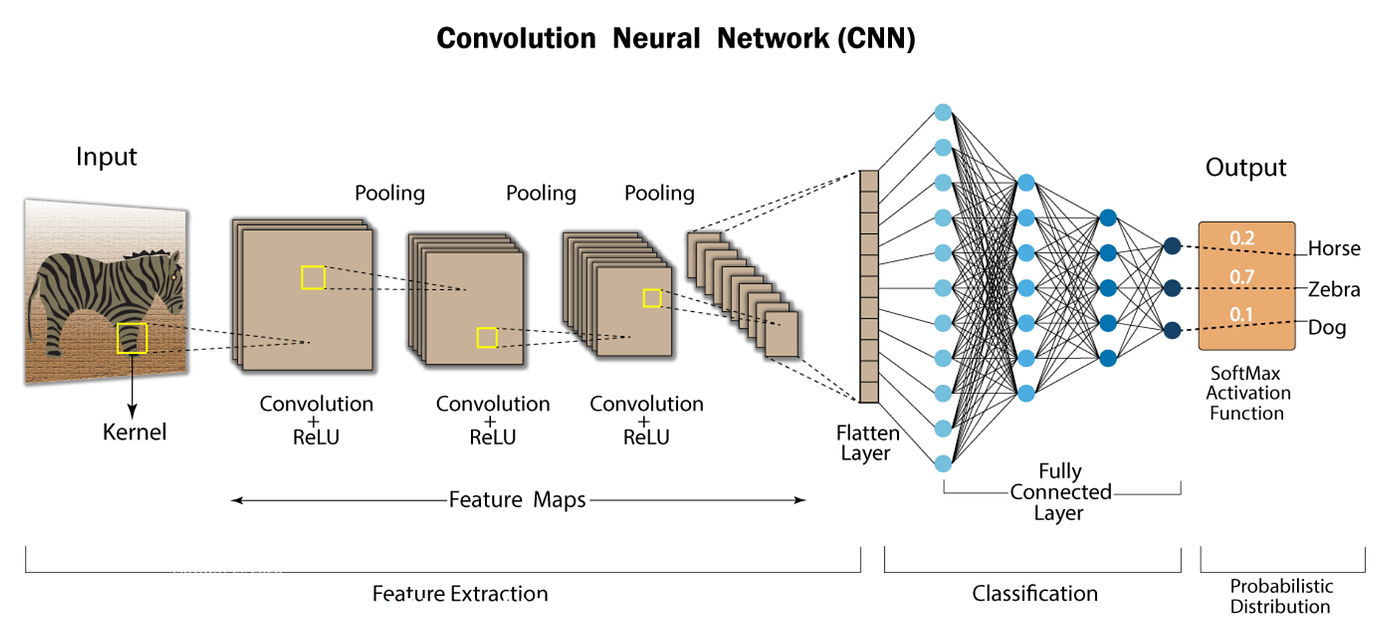
\includegraphics[width=0.6\textwidth]{images/cnn_architecture.png}
  \end{figure}
\end{frame}